\documentclass{article} % For LaTeX2e
\usepackage{nips14submit_e,times}
\usepackage{hyperref}
\usepackage{url}
\usepackage{amsmath}
\usepackage{amsfonts}
\usepackage{graphicx}
%\documentstyle[nips14submit_09,times,art10]{article} % For LaTeX 2.09


\title{ECE285 Project Progress Report: High Speed Imaging with Compressed Sensing}


\author{
Yingwei Li*, Huan Hu* \\
\AND huh015@eng.ucsd.edu
}

% The \author macro works with any number of authors. There are two commands
% used to separate the names and addresses of multiple authors: \And and \AND.
%
% Using \And between authors leaves it to \LaTeX{} to determine where to break
% the lines. Using \AND forces a linebreak at that point. So, if \LaTeX{}
% puts 3 of 4 authors names on the first line, and the last on the second
% line, try using \AND instead of \And before the third author name.

\newcommand{\fix}{\marginpar{FIX}}
\newcommand{\new}{\marginpar{NEW}}

\nipsfinalcopy % Uncomment for camera-ready version

\begin{document}


\maketitle

\begin{abstract}
In this course project, we plan to build a mathematical model for high speed imaging system with compressed sensing. Due to the sparseness of the underlying image, compressed sensing can be applied in the image reconstruction. We'll conduct simulations for a full-functioning imaging system and analyze the results for further improvements.
\end{abstract}

\section{Literature Review}
We review a few papers related to compressive imaging systems. In particular, we're interested in the recovery problem formulation , sensing matrix design and algorithms to solve the problem.
\subsection{SparseMRI}
\subsubsection{recovery problem formulation}
[2] introduces a method for fast Magnetic Resonance Imaging(MRI). The measurement matrix in MRI system is random partial DFT matrix and the sparsity assumption can be made in either the imaging space or wavelet space. Specifically, we need to solve the inverse problem:
\begin{align*}
b&=A x \\
&subject~to~ \alpha=\Phi x,\alpha~is~sparse
\end{align*}
where A is the random partial DFT matrix and $\Phi$ is the domain where the image is sparse(can be either the original image domain or the wavelet matrix).

This inverse problem can be solved with guarantee by L1 minimization since partial DFT matrix satisfy RIP conditions. That is,
\begin{align*}
x^*&=argmin |\Phi x|_1 \\
&subject~to~|b-Ax|_2<\epsilon
\end{align*}
One thing that's particular interesting to our project is that, changing the L1 objective function to \textbf{Total Variation (TV)} is closed related to sparsity assumption in wavelet space. More generally, even if the sparsity domain is not wavelet space, a TV term can also be added to enforce smoothness. [We hope this is useful in our imaging system.]
\begin{align*}
x^*&=argmin |\Phi x|_1+\lambda TV(x) \\
&subject~to~|b-Ax|_2<\epsilon\\
&where~TV(x)=|D(x)|, D(x)~ is~ the~discrete~differential~operator. 
\end{align*}

\subsubsection{discussions about sensing matrix}
As the paper discusses, the validity of compressive sensing in MRI largely depends on the nice property of the sensing matrix, which is partial DFT matrix. In their discussion, an intuitive heuristic guideline for evaluation of the sensing matrix is defined. As we desire \textbf{incoherent artifacts caused by undersampling}, a natural measure would be the \textbf{Point Spread Function(PSF)} as defined in the paper. Actually, this definition is exactly the mutual coherence of a matrix which is discussed in our early lectures. We know it can lead to sufficient conditions for exact recovery. 

Thus, we would like to experiment with minimization of mutual coherence of the sensing matrix in our imaging system, although we're given limited freedom of choice(the sensing matrix is related to the optical properties and layout of the materials in the system).

The paper also discusses a lot about the sampling strategy considering smooth sample trajectories due to hardware and physiological limitations. Moreover, their system also has a "calibration" step to correct phase misalignment, which is similar to our system.

\subsection{Single-Pixel Imaging}
\subsubsection{hardware architecture}
In [1], the author describes a full-blown imaging system with only a single photon detector.  The system is mainly composed of biconvex lenses, a DMD(digital micromirror device) spatial light modulator , a single photon detector and a A/D converter. This whole architecture is essentially a optical computer. Since the DMD is programmable, the system can get M random measurement of the scene by generating different patterns and take the inner product with the image. With sufficiently large number of measurement(M= O(K log(N/K))), we're guaranteed to have exact imaging result. 
\subsubsection{recovery problem formulation}
The formulation is very similar to MRI case, except with a different sensing matrix. Also, this system uses the TV formulation in addition to L1 minimization.
\subsubsection{sensing matrix design}
The system uses random rows of 0/1 Walsh matrix as the sensing matrix. But the paper also suggests Hadamard or noiselet transform. These are all sampled rows from a deterministic matrix instead of the i.i.d Gaussian case discussed in our lectures.
\subsubsection{image classification by smashing filter}
The paper demonstrates one interesting experiment of image classification. They argue that the naive approach would first reconstruct the full image and then do classification in the original image space $R^n$. The smashed filter exploits a recent result that the structure of a smooth k-dimensional manifold in $R^n$ is preserved with high probability under a random projection to the lower dimensional space $R^m$ as long as m = O (k log n ). (note this is quite similar to the guarantee of exact recovery of sparse signal although here it's a subspace). With this guarantee, the smashed filter performs all the operations on the measurements directly without recovery of the full image.

The paper shows that with more measurements, the accuracy of classification by smashed filter increases, which satisfies our intuition.

\section{Experiments Results of Our System}
\subsection{different design of sensing matrix $A$}
Based on the underlying theory of photonics, we simulate two settings of the sensing matrix.($A1$ and $A2$) (we leave out the technical details here). 
Both $A1$ and $A2$ are generated by randomly placing light sources on our optical material hence has some randomness(the exact distribution is unknown due to complex physical interaction). An example of $A1$ and $A2$ is shown in Figure 1 and Figure 2 respectively.

 For $A1$, the sensing structure is relatively simpler and can only sensing one dimension of the underlying image(i.e. determine if \textit{any} pixel in a column is non-zero). figure[??] shows an example of L1 recovery result.
 
From our experiment, with $A1$ of size $30 \times 80$, sparsity 10,image size 80, the system is quite reliable to recover the original image. This is a promising result.

For $A2$, we include more complex layout strategy for the light sources hence resulting sensing matrix that can sense 2-D images. Figure 2 shows an example of the recovery result.

We compare two different algorithms for solving the L1 minimization problem. One provided by [4] which is a l1-Regularized Least Squares method. The other is termed as \textbf{smoothed L0 norm (SL0)}[5] which tries to directly minimize the L0 norm with a approximation function (in our experiment SL0 performs better).

From our experiment, with $A2$ of size $160 \times 400$, sparsity 20, image size $20 \times 20$, the system can successfully recover the original image. 

\begin{figure}[!t]
\centering
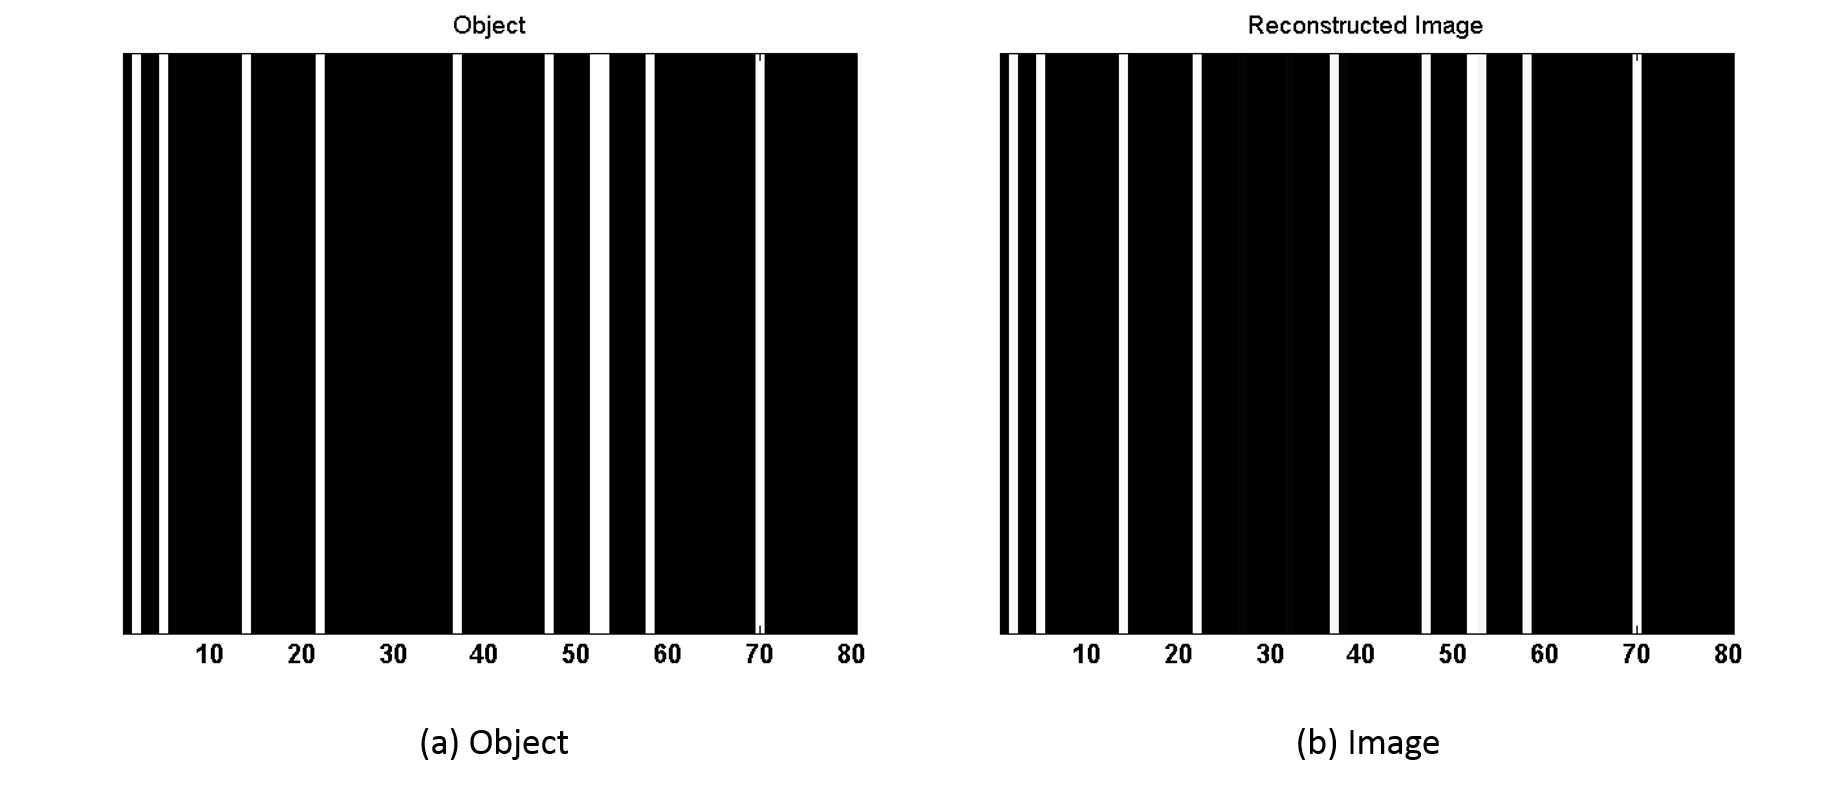
\includegraphics[width=5in]{5.png}
% where an .eps filename suffix will be assumed under latex,
% and a .pdf suffix will be assumed for pdflatex; or what has been declared
% via \DeclareGraphicsExtensions.
\caption{A1: 1D imaging computational experiment }
\end{figure}

\begin{figure}[!t]
\centering
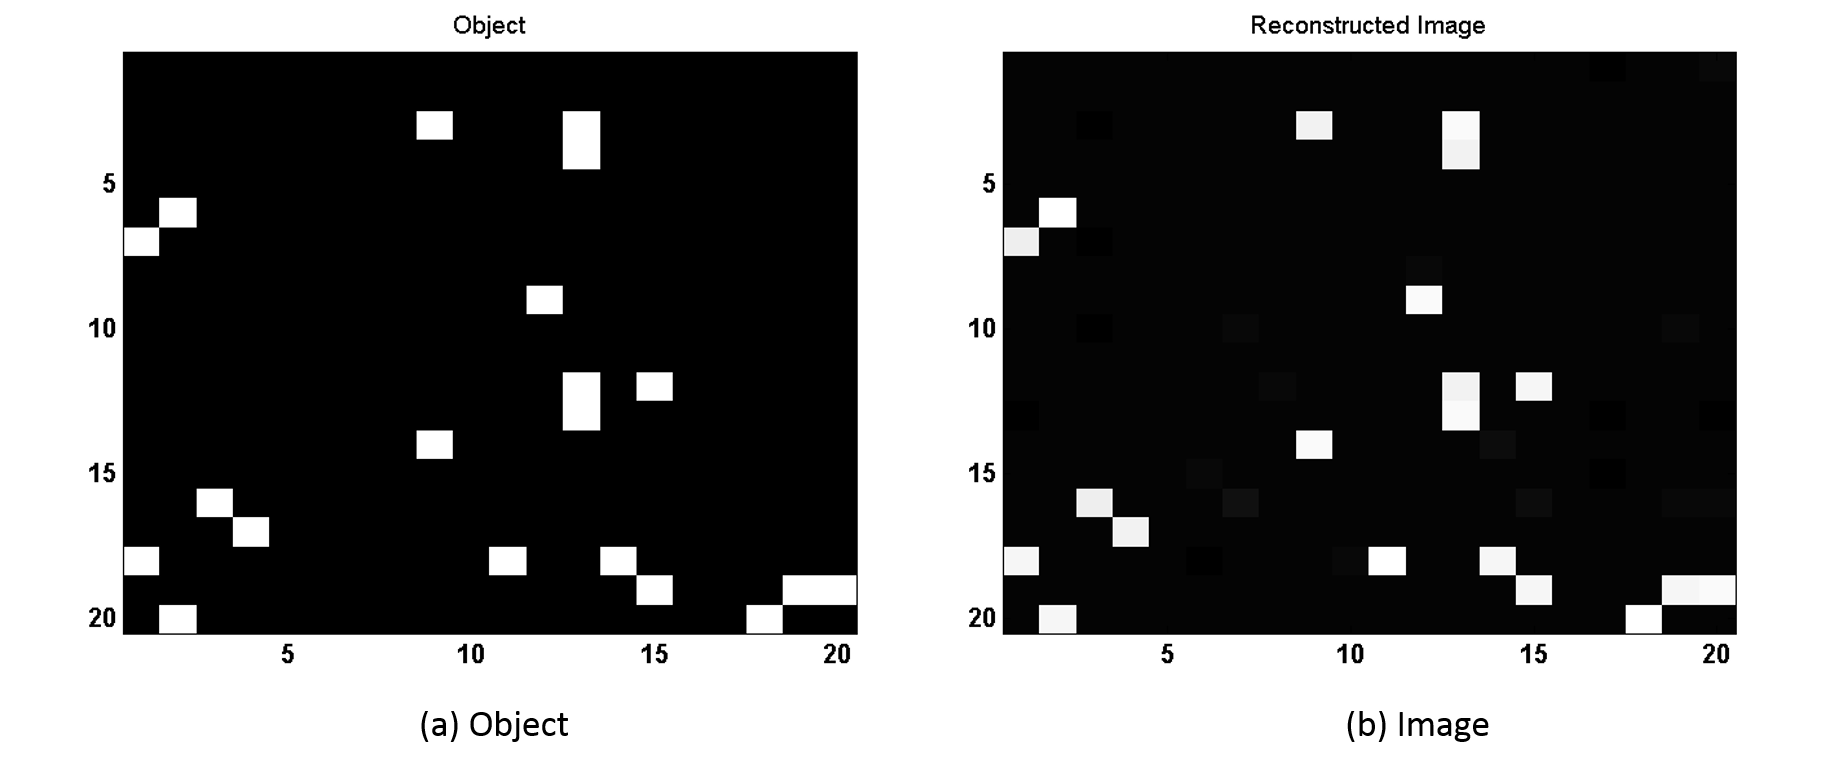
\includegraphics[width=5in]{6.png}
% where an .eps filename suffix will be assumed under latex,
% and a .pdf suffix will be assumed for pdflatex; or what has been declared
% via \DeclareGraphicsExtensions.
\caption{A2: 2D imaging computational experiment }
\end{figure}

\section{Future Work}
Based on the review of the imaging systems, we would like to experiment with our system in the following aspects:

\begin{enumerate}
\item We'll try to add TV norm minimization to our current system. As in the other existed imaging systems, this assumption will lead to smooth images.
\item Also, we'll try to find the optimal layout of the optical material so that the sensing matrix is most "incoherent". 
\item To solve sparse recovery problems, a lot of solvers are available online, each with different approaches to relax the original L0 problem. We'll continue to evaluate their performance with respect to imaging quality in our system and hopefully will find the optimal one for our purpose.
\end{enumerate}

\vspace*{3\baselineskip}

\small{
[1] Willett R M, Marcia R F, \&Nichols J M. Compressed sensing for practical optical imaging systems: a tutorial[J]. {\it Optical Engineering}, 2011, 50(7): 072601-072601-13.

[2] Lustig, Michael, David Donoho, \& John M. Pauly. "Sparse MRI: The application of compressed sensing for rapid MR imaging." {\it Magnetic resonance in medicine 58.6 (2007)}: 1182-1195.

[3] Duarte M F, Davenport M A, \&Takhar D, et al. Single-pixel imaging via compressive sampling[J]. {\it IEEE Signal Processing Magazine}, 2008, 25(2): 83.

[4] Koh K, Kim S J, Boyd S P. An interior-point method for large-scale l1-regularized logistic regression[J]. Journal of Machine learning research, 2007, 8(8): 1519-1555.

[5] Mohimani, G. Hosein, Massoud Babaie-Zadeh, \& Christian Jutten. Complex-valued sparse representation based on smoothed ? 0 norm. {\it Acoustics, Speech and Signal Processing, 2008. ICASSP 2008. IEEE International Conference on.} IEEE, 2008.

%[1] Alexander, J.A. \& Mozer, M.C. (1995) Template-based algorithms
%for connectionist rule extraction. In G. Tesauro, D. S. Touretzky
%and T.K. Leen (eds.), {\it Advances in Neural Information Processing
%Systems 7}, pp. 609-616. Cambridge, MA: MIT Press.
%
%[2] Bower, J.M. \& Beeman, D. (1995) {\it The Book of GENESIS: Exploring
%Realistic Neural Models with the GEneral NEural SImulation System.}
%New York: TELOS/Springer-Verlag.
%
%[3] Hasselmo, M.E., Schnell, E. \& Barkai, E. (1995) Dynamics of learning
%and recall at excitatory recurrent synapses and cholinergic modulation
%in rat hippocampal region CA3. {\it Journal of Neuroscience}
%{\bf 15}(7):5249-5262.
%}

\end{document}
